\section{Chapter Overview}

%  Even though many people have got into purchasing \Gls{nft}s, one of the major problems that owners, as well as potential customers face, is that they’re unable to find NFTs that are worth trading their current NFTs to.
 In this research project, the author tries to identify the required features to be considered for an NFT-trading Recommendations System and introduce a new Ensemble Architecture for Recommendations that can be applied in other related domains as well. The proposed architecture will try to automate several decision-making steps that a user would otherwise need to go through to find the best possible trade.

This chapter defines the problem, the research gap, the research challenge, and the research strategy that the author wishes to follow over the next few months. The necessary proofs of the problem, as well as previous research interests, are also reviewed.

% Methodologies chapter - Finally, in the Work Plan, the expected schedule of the project's deliverables is presented.

\section{Problem Domain}
\vspace{2mm}
\subsection{Non-fungible Tokens (NFTs)}
In recent months, the \Gls{nft} market has been growing exponentially as it appears to be the most widely accepted business application of Blockchain technology \autocite{dowling_is_2021}, since the introduction of crypto.
\Gls{nft}s are provably scarce unique digital assets that can be used to represent ownership \autocite{noauthor_erc-721_nodate}.
They can be one of a kind rare artworks, collectable trading cards, and other assets with the potential to increase in value due to scarcity \autocite{conti_what_2021, fairfield_tokenized_2021}. While being digital assets, they also can be used to represent physical assets. A digital certificate of land/ qualification can be identified as a couple of examples. The biggest winners in the NFT space over the last few months have been digital artists who were able to sell art worth over \$2.5 Billion \parencite{noauthor_off_2021}.


NFTs were introduced by Ethereum \autocite{wood_ethereum_2014} as an improvement proposal \autocite{noauthor_eip-2309_nodate, noauthor_erc_nodate} in the \gls{erc}-721 standard \autocite{noauthor_erc-721_nodate}. This allows anyone to implement a Smart Contract with the ERC-721 standard and let people mint NFTs as well as, keep track of the tokens produced by it. This allows the created tokens to be validated.

% \bigbreak
% Smart Contracts
Each of these created tokens is unique from the other tokens created by the same Smart Contract, unlike fungible tokens which were introduced with cryptocurrencies and are denoted by the ERC-20 standard \autocite{noauthor_erc-20_nodate} on the Ethereum network. One Bitcoin can be swapped to another Bitcoin, but each NFT will be unique.
Then, the deployed Smart Contract will be responsible to keep track of the tokens created by it on the network. A Smart Contract is a program that resides on the Ethereum network with a collection of code \& data \autocite{noauthor_introduction_nodate}.

For each NFT, the contact address \& unit256 tokenId are globally unique on any blockchain. This allows Decentralized Applications (DApps) \autocite{frankenfield_decentralized_nodate, noauthor_decentralized_2021} to take the tokenId and present the image/ asset that is identified by the particular NFT.

% \bigbreak
\emph{"To put it in terms of physical art collecting: anyone can buy a Monet print. But only one person can own the original."} \autocite{clark_people_2021}

While a digital file can be copied regardless of whether it's an NFT or not, what this technology provides is the ownership of the digital asset.
% That is something that cannot be copied or taken from the owner. 
If an NFT that contains your certificate/ domain is held under your wallet on the Blockchain, no one else can get it from you unless they have your digital wallet's private key. Similar to a deed. But, anyone can see, validate and admire what you own.

% ----------------

\subsection{NFT Marketplaces}

% NFT Market places & what they offer. 

% Money in NFT & how markets have expanded (Open sea used by Reddit NFTs) and been funded.
OpenSea, which was the first NFT marketplace is also considered to be the largest. In the attempt to become the "Amazon of NFTs", OepnSea raised \$23 million in a Series A \autocite{hackett_this_2021}, following a \$100 million raise in a Series B round, ended the company in a valuation of \$1.5 billion \autocite{dfinzer_announcing_2021, matney_nft_2021}. Open Sea saw nearly \$150 million in sales in the month of June.
These marketplaces are set to increase access to the digital goods industry \autocite{chevet_blockchain_2018}.


An NFT purchased on an Ethereum marketplace can be traded on any other Ethereum marketplace for a completely different NFT. Creators don't necessarily need to sell their NFT on a market. They can do the transaction peer-to-peer, completely secured by Blockchain. No one is needed to intermediate and an owner isn't locked onto any platform \autocite{noauthor_erc-721_nodate}.

% How they can benefit from Recommendations - add to motivation? - already mentioned in problem

\subsection{Recommendation Systems}
Recommendation Systems have been driving engagement and consumption of content as well as items on almost every corner of the internet over the last decade.
% \bigbreak
These systems help users identify relevant items on an online platform. When users are recommended with relevant items, it enables businesses in growing their revenue. 35\% of Amazon’s revenue \autocite{naumov_deep_2019} \& 60\% of watch time on YouTube \autocite{noauthor_recommendations_nodate} comes from recommendations.


% ***\section{Problem Domain}
% Furthermore, they have to refer to several sources across the internet to find items that are highly trending.



% Although Computer Scientists and Data Scientists have pushed the limits of Recommendation Systems with recent advances in Machine Learning and Deep Learning, it is clear that none of the currently available Recommendation Architectures satisfies the thinking process identified by NFT owners & potential customers when searching for NFTs to trade.


\section{Problem Definition}
Currently, there is no way of identifying possible tradable NFT assets, unless manually browsing through the internet. 
Marketplaces allow searching for NFTs by keywords, categories \& pricing, but don't provide personalized recommendations of trending items.
This applies to someone who wants to purchase an NFT that shows similar characteristics to another NFT that has already been purchased by a previous buyer or oneself. Since there can be only one owner for an NFT at a time, recommendations using standard collaborative filtering is also not entirely ideal. Content-based approaches won't help identify trending items.

\bigbreak
To help with the exploration of these digital assets, it's identified that several steps that the user has to follow to identify trending items that are timely, popular among the community and may have an expected value can be automated. 

\subsection{Problem Statement}
It is difficult to find NFTs of comparable value that is trending among the community, timely and relevant to the user’s identified interest or the NFT that the user currently owns.

\section{Research Motivation}
% This has to be to the point!!!!
%  Refer to why it's important to solve this problem in NFTs
The problem identified in this proposal applies to both people who have a lot of domain knowledge about \gls{nft}s and people who have no idea how valuable items are in relation to their interests. Whoever it is, no solution would mimic the exact thinking pattern of a person who is searching for a suitable \gls{nft}.

As mentioned in the work of \textcite{cheng_hybrid_2020}, Recommendation Systems play a significant role in the resolution of the problem of information overload. In order to provide ideal recommendations to a user, it is important to understand the user's thought process as well as other factors that affect a decision to trade.

Since the Recommendations domains are highly important for many business use-cases and the \gls{nft} domain is seeing a booming acceptance with a bright future ahead, this work is expected to add value to the progression of advancements \& accessibility related to the domains of \gls{nft}s, Blockchain \& Recommendation Systems.

% group is broken here to prevent end of line going to the next page
\newpage
\section{Related Work}

% \subsection{Recommendation Systems}
% \centering
\vspace{-4mm}
\begin{longtable}{|p{0.17\linewidth}|p{0.18\linewidth}|p{0.27\linewidth}|p{0.27\linewidth}|} 
% check the error here
\caption{Related work in Recommendations Systems}
\label{tab:related-work-table}\\
\hline
Citation & Technique Used & Improvements & Limitations \\ 
\hline
\autocite{larry_history_2019} & Autoencoder, trained on chronologically sorted movie-viewing data & Outperformed item-to-item collaborative filtering \& the bestseller list & \textit{Critique: The timeline doesn't consider overlapping of movies at various points in time, which will be necessary for trends.~}Tested only on movie recommendations. \\ 
\hline
\autocite{cheng_hybrid_2020} & A framework that integrates collaborative filtering with opinion mining \& sentiment analysis on users' reviews that is used to create preference profiles. & Effective in dealing with insufficient data and is more accurate and efficient than existing traditional methods. The quality of recommendations can be improved regardless of whether the dataset is rich or sparse. & The semantic strategy of opinion extraction is generic. This may not be ideal to identify different aspects in varied genres. Slang, irony or sarcasm isn't considered in the current framework. It's very dependent on text mining of user reviews.~\textit{Critique: A person has to have placed reviews on previous movies in order to create a preference profile.} \\
\hline
\autocite{chen_user_2019} & A deep learning model to process user comments and to generate a possible user rating for user recommendations have been used. & Outperforms baseline models in training loss value, precision, and recall on the Yelp and Amazon data sets. In the Trip-Advisor data set, DBNSA (Deep Belief Network and Sentiment Analysis) has the best MSE training loss value and recall.

DBNSA saves more time than the other baseline methods. & At present, the proposed method is not suitable for real-time testing. This method is required to be tested with a fast Deep Learning algorithm. Sarcastic comments have not been considered in user comments. \\ 
\hline
\autocite{ayushi_cross-domain_2018} & A hybrid approach of combination of content-based recommendation, user-to-user collaborative filtering and personalized recommendation techniques. & Address the limitations of single domain analysis such as data sparsity and cold start problem.

Integration of several domains is further capable of generating higher accuracy in suggestions.

Twitter sentiment analysis over the recommended entities generated by the model to help the user in decision making by knowing the positive, negative and neutral polarity percentage based on tweets done by people. & \textit{Critique: Sentiment analysis based on Twitter sentiment is calculated and shown after showing recommendations. It's ironic to recommend something and say if it's good/ bad by the system itself. Better if only positive sentiment-based items are recommended. }\\ 
\hline
\autocite{ferdiansyah_lstm-method_2019} & LSTM (Long short-term memory). & The proposed model with time series techniques can predict the price for the next days with split the data to train and test. & The result is not good enough regarding the RMSE (Root Mean Squared Error). Future work: modified LSTM layers, adding dropout and modified number of epochs, and using different instability data-sets to test how good the prediction results are or~\textit{try to use sentiment analysis combined with LSTM method}~to see the impact of the uncertainty in value bitcoin. \\ 
\hline
\parencite{noauthor_what_2020} & Multiple Regression & This considers past purchase patterns, NFTs saved in wallets to predict if another wallet containing a similar combination will be likely to own an NFT from a specific category (eg: Cryptokitties, ENS domains, etc) in the future. & Recommends NFT categories that a user may be interested in. Doesn't recommend specific NFTs. The user needs to either manually input preferences or provide his wallet key that contains all his owned assets.~\textit{Critique: This won't consider current trends. It won't consider the recognition of the creators (eg: NFT made by Beeple).} \\
\hline
\end{longtable}

% \begingroup
% \let\clearpage\relax
% Public Opinion - cheapest to get from social media & google trends

% ?***Crypto predictions using twitter data
% Abraham, J., Higdon, D., Nelson, J., Ibarra, J., 2018. Cryptocurrency Price Prediction Using Tweet Volumes and Sentiment Analysis 1, 22.
%? Netlify representation of recommendations

% ***this subsection might have to be changed?
% \subsection{Understanding factors that affect NFT Markets}
% % Facts to be considered related to NFTs when recommending
% % \autocite{noauthor_off_2021} - price of NFTs have a relationship between the hype of the society and the interests of the community.
% It is understood that the pricing of NFTs is moved by the changes in the pricing of cryptocurrencies, but appears to have comparatively less volatility. But the spillover between NFT markets has been identified to be very low compared to the high spillover effect among individual crypto markets \autocite{dowling_is_2021}.

% The very first study done examining the pricing of NFTs suggests that \emph{"prospects for future studies are potentially limitless, as at the beginning of any new market"} \autocite{dowling_fertile_2021}. As a future study, the author has suggested identifying if there's a fundamental model that drives the price determination in NFTs.

% \begin{quote} 
% \centering 
% \emph{"The value of an NFT is entirely determined by what someone else is willing to pay for it."}
% \\
% \raggedleft
% \autocite{conti_what_2021}
% \end{quote}

% \begin{quote} 
% \centering 
% \emph{"Ultimately owning the real thing is as valuable as the market makes it. The more a piece of content is screen-grabbed, shared, and generally used the more value it gains. Owning the verifiable real thing will always have more value than not."}
% \\
% \raggedleft
% \autocite{noauthor_erc-721_nodate}
% \end{quote}


% These statements prove that the demand for investment in NFTs will be heavily reliant on the public's acceptance of the item is.

% ----------------


% \begingroup
% \let\clearpage\relax 
% summarize & point out why research is required
% Considering the above-mentioned points, 
\section{Research Gap}
Based on previous work done related to Recommendation Systems, the literature doesn't identify integrating all the factors that affect the desirability of owning relevant, timely \& trending NFTs (items) to a recommendations model. This project focuses on an Empirical gap in the NFT domain as well as Theoretical and Performance gaps in Recommendations Systems. 
% Empirical gap - research that is based on observation and measurement of phenomena, as directly experienced by the researcher. 

Collaborative filtering, which has been a standard baseline technique for Recommendations for over a decade, can't be taken as the only recommendations model because, by the time one NFT is viewed many times by other users, it may already be too late for another user to purchase that item.


\section{Research Contribution}

% *** this will come to a solution? The main challenge when it comes to recommending NFTs to users is that the Recommendations System has to know what items are trending in the world while being relevant.

% \bigbreak
The author's research contribution can be summarized as follows:
\begin{itemize}
\item \textbf{Recommendations Systems}: Data Engineering + Data Science [\Gls{ml} + \Gls{dl}] + Ensemble models
\item \textbf{NFT Trading}: Recommendations + \Gls{ai} + Automation + Data Analysis
\end{itemize}

\subsection{Technological Contribution}

A Hybrid Recommendations technique that attempts to use public trends in a way that hasn't been attempted in previous research will be explored in order to facilitate the recommendation of relevant, trending and timely items. Automation of several decision-making steps that a user would otherwise need to go through to find the best possible trade will be integrated into the Recommendations Architecture. It is hypothesized that this novel recommendations architecture will be able to be applied to other items as well to give enhanced recommendations based on trends.

\subsection{Domain Contribution}

The information in an NFT that has an effect on a user's desire to be owned will be identified, when attempting to provide suitable recommendations.
Looking at the success of Recommendation Systems across multiple systems for over a decade, it is understood that a Recommendation System would help users identify NFTs that they would be interested in trading. This will in return help in increasing sales on NFT Marketplaces and wider adoption of the technology.

\bigbreak
NFTs are a result of the advancement of the application of techniques related to Blockchain, while Recommendation Systems are a result of Data Science advancements over the last few decades. Both the domains considered in this research can be identified to be originated from the field of Computer Science.


\section{Research Challenge}
NFTs is a new domain, which has very less research done related to preferences and factors considered when purchasing NFTs.
Therefore, it is first important to identify the data points (features) \& external factors that affect the value/ desirability of owning NFTs to suggest trading recommendations of NFTs to a user.

\bigbreak
% add this to challenge?
\textit{"Crypto has a founding tradition of emphasizing freedom and privacy. Maybe because of this prevailing cultural trend, the NFT space does not have many recommender systems."} \autocite{noauthor_what_2020}

NFTs are identified to be more challenging to be recommended to users using traditional recommendation methods due to the uniqueness of each item together with the traditions brought forward with the crypto community.
Similar to cryptocurrencies, it has been identified that NFTs too have an impact on the general public opinion \& trends \autocite{dowling_fertile_2021}.

Currently, available Recommendation Systems haven't had the necessity to consider trends as much as with related to the desirability of owning NFTs. Furthermore, scarcity of items opens another challenge of the inability to keep recommending items that are not available for sale or have already been purchased by an interested buyer. But that alone can't be considered due to the time-tested \& proven baseline recommendation techniques being highly effective in multiple domains. Using the identified factors to be considered, a suitable recommendations architecture needs to be implemented.

\section{Research Questions}

\begin{itemize}[label={}]
  \item {\textbf RQ1:} What are the features of NFTs \& external factors that affect the desirability of owning NFTs?
  \item {\textbf RQ2:} How can a system predict the most relevant, trending, timely \& worthy NFTs for trading purposes?
  \item {\textbf RQ3:} What are the recent advancement in recommendation models \& architectures that can be taken into consideration when building a hybrid Recommendation Architecture, using ensemble techniques? 
\end{itemize}

\section{Research Aim}
\textit{The aim of this research is to design, develop \& evaluate a novel Recommendation Architecture that will provide relevant, trending, timely, and worthy NFTs for trading purposes by automating some of the decision making steps that the user would otherwise have to do manually.}

\bigbreak
To elaborate on the aim, this research project will produce a system \& architecture that can be used to recommend trending items with respect to a chosen item in a specific data set. The focus will be laid on the recommendation of NFTs. In order to achieve this several public channels of trends will be required to be streamed into the recommendations architecture together with the automation of several decision-making steps that a user that is interested in purchasing NFTs would have to manually go through, in order to make the best possible trade. The use of Data Mining techniques, \Gls{nlp} techniques, Data Analysis, hybrid, content-based, collaborative filtering \& Deep Learning methods will be researched to make the best possible recommendations.

The required knowledge will be studied and researched, components will be developed and the performance will be evaluated in order to validate or invalidate the chosen hypothesis. The system will be able to run in a local browser for personal use or in a hosted server for public use. The data science models \& their code will be available for further research and use in a public repository that is easy to get up and running with ease. A review paper will be published with knowledge gathered from the survey of Literature. A research paper will be published on the outcome of the findings in the research project.

\section{Research Objectives}
The Aims and Research Questions mentioned above are expected to be achieved and answered with the completion of the following Research Objectives. These objectives are milestones that will be expected to be met in order for the research to be completed successfully.

\newpage
% \vspace{-4mm}

% breakdown all the rows into atomic objectives to be done
% \begin{table}[h!]
% \centering
\begin{longtable}{| p{0.135\linewidth} | p{0.63\linewidth}| p{0.12\linewidth}| p{0.04\linewidth}|}
\caption{Research Objectives}
\label{tab:research-objectives-table}\\
\hline
Objective &   Description & Learning Outcomes & RQ \\ 
\hline
% Problem Identification & Identifying a suitable and valuable problem domain to contribute towards, with identified research gaps suitable for a research project.
% & LO5 \\
% \hline
Literature Survey & Read previous work to collate relevant information on related work and critically evaluate them.
\begin{itemize}
\item \textbf{RO1:} Conduct a preliminary study on existing Recommendations Systems \& Architectures.
\item \textbf{RO2:} Analyze the perception of Recommendation techniques.
\item \textbf{RO3:} Conduct a preliminary study on \Gls{nft}s.
\item \textbf{RO4:} Analyze user desires and factors that affect the likability of owning \Gls{nft}s.
\vspace{-7mm}       % remove line spacing after itemize
\end{itemize}
& LO4, LO2, LO5 
& RQ1 RQ3
\\
\hline
% Project Methodology & Choosing the Research, Development and Project Methodologies that can be followed. Creating a project plan with expected activities and scheduled times for the time frame allocated for the project.
% & LO3, LO7 \\
% \hline
Requirement Analysis &  Specifying the requirements of the project using appropriate techniques and tools in order to meet the expected research gaps \& challenges to be addressed based on previous related research and any domain-specific sources of knowledge.
\begin{itemize}
\item \textbf{RO5:} Gather information about requirements related to desirability of owning \Gls{nft}s \& crypto-related assets.
\item \textbf{RO6:} Gather the requirements of a Recommendations System and understand end-user expectations.
\item \textbf{RO7:} Get insights \&  opinions from technology \& domain experts to build a suitable system.
\vspace{-7mm}       % remove line spacing after itemize
\end{itemize}
& LO1, LO2, LO5, LO7 
& RQ1 RQ2 RQ3
\\
\hline
Design & Designing architecture and a system that is capable of solving the identified problems with recommended techniques.
\begin{itemize}
\item \textbf{RO8:} Design a price prediction system to identify the possible increase/ decrease in value of the \Gls{nft}s.
\item \textbf{RO9:} Design an automated flow to match \Gls{nft}s with global social trends data.
\item \textbf{RO10:} Design a data-preprocessing pipeline to add Smart Contract data related to \Gls{nft}s in the system.
\item \textbf{RO11:} Design a \Gls{dl} or \Gls{ml} Recommendations model that is capable of appropriately utilizing feature-enhanced data to produce recommendations.
\vspace{-7mm}       % remove line spacing after itemize
\end{itemize}
& LO1 
& RQ2 RQ3
\\
\hline
Development & Implementing a system that is capable of addressing the gaps that were aimed to be solved. 
\begin{itemize}
\item \textbf{RO12:} Develop a Recommendations System that can produce relevant, timely \& trending NFTs (items).
\item \textbf{RO13:} Integrate automation steps in the prototype to enhance features of NFT records and use them to recommend suitable NFTs.
\item \textbf{RO14:} Develop an algorithm that can utilize factors that are considered to affect the desirability of owning an NFT by a person.
\vspace{-7mm}       % remove line spacing after itemize
\end{itemize}
& LO1, LO5, LO6
& RQ1 RQ2 RQ3
\\
\hline
Testing and Evaluation & Testing the created system \& Data science models with appropriate data and evaluating them with baseline techniques identified in the literature. 
\begin{itemize}
\item \textbf{RO15:} Create a test plan and perform unit, integration and functional testing.
\item \textbf{RO16:} Evaluate the novel model by bench-marking with  \Gls{p@k} score, compared against baseline models.
\vspace{-7mm}       % remove line spacing after itemize
\end{itemize}
& LO4
& RQ1 RQ2 RQ3
\\
\hline
Documenting the progress of the research & Documenting and notifying the continuous progress of the research project and any faced obstacles. 
& LO8, LO6
& RQ1 RQ2
\\
\hline
Publish Findings & Produce well-structured documentation/ reports/ papers that critically evaluate the research.
\begin{itemize}
\item \textbf{RO17:} Publishing a review paper on related work.
\item \textbf{RO18:} Publishing evaluation \& testing results identified from the research.
\item \textbf{RO19:} Making the code or models created in the research process available for future advancements in research.
\item \textbf{RO20:} Making any modified data-sets or re-creation strategies available to the public, to train \& test models related to similar use cases of utilized data.
\vspace{-7mm}       % remove line spacing after itemize
\end{itemize}
& LO4, LO8
& RQ1 RQ2 RQ3
\\
\hline
\end{longtable}
% \end{table}


\section{Project Scope}
The scope is defined as follows based on the project objectives and a review of existing products with consideration to the granted time period for this research project.

\subsection{In-scope}
The following is a list of the project's scope:
\begin{itemize}
\item A system that is capable of recommending NFTs to users based on a specific chosen \gls{nft}.
\item Creation of a Recommendations System that integrates public trends on social media.
\item Creation of a Recommendations System that is capable of providing better rending recommendations compared to baseline techniques.
\item Testing the requirement of integrating public trends into a Recommendations architecture with the use of Content-based filtering, collaborative filtering \& Deep Learning techniques.
\item \Gls{gui} that allows a user to provide the tokenId of a chosen NFT by the user \& to view the results given by the Recommendations System.
\item Automation techniques with related to Smart Contracts will be directly applicable only to selected Blockchains.
\end{itemize}

\subsection{Out-scope}
The following are the parts that will not be covered by the project:
\begin{itemize}
\item Recommending items that haven't been seen previously by the system.
\item Creating a Recommendations System that utilizes less computational power \& resources compared to baseline techniques.
\item GUI with options to tune the Recommendations System.
\item All automation techniques to cover every available Blockchain.
\end{itemize}

\subsection{Prototype Diagram}
% \vspace{-7mm}       % remove spacing
% this diagram has gone to a different place after line spacing adjustment
\vspace{-4mm}
\begin{figure}[ht!]
\centering
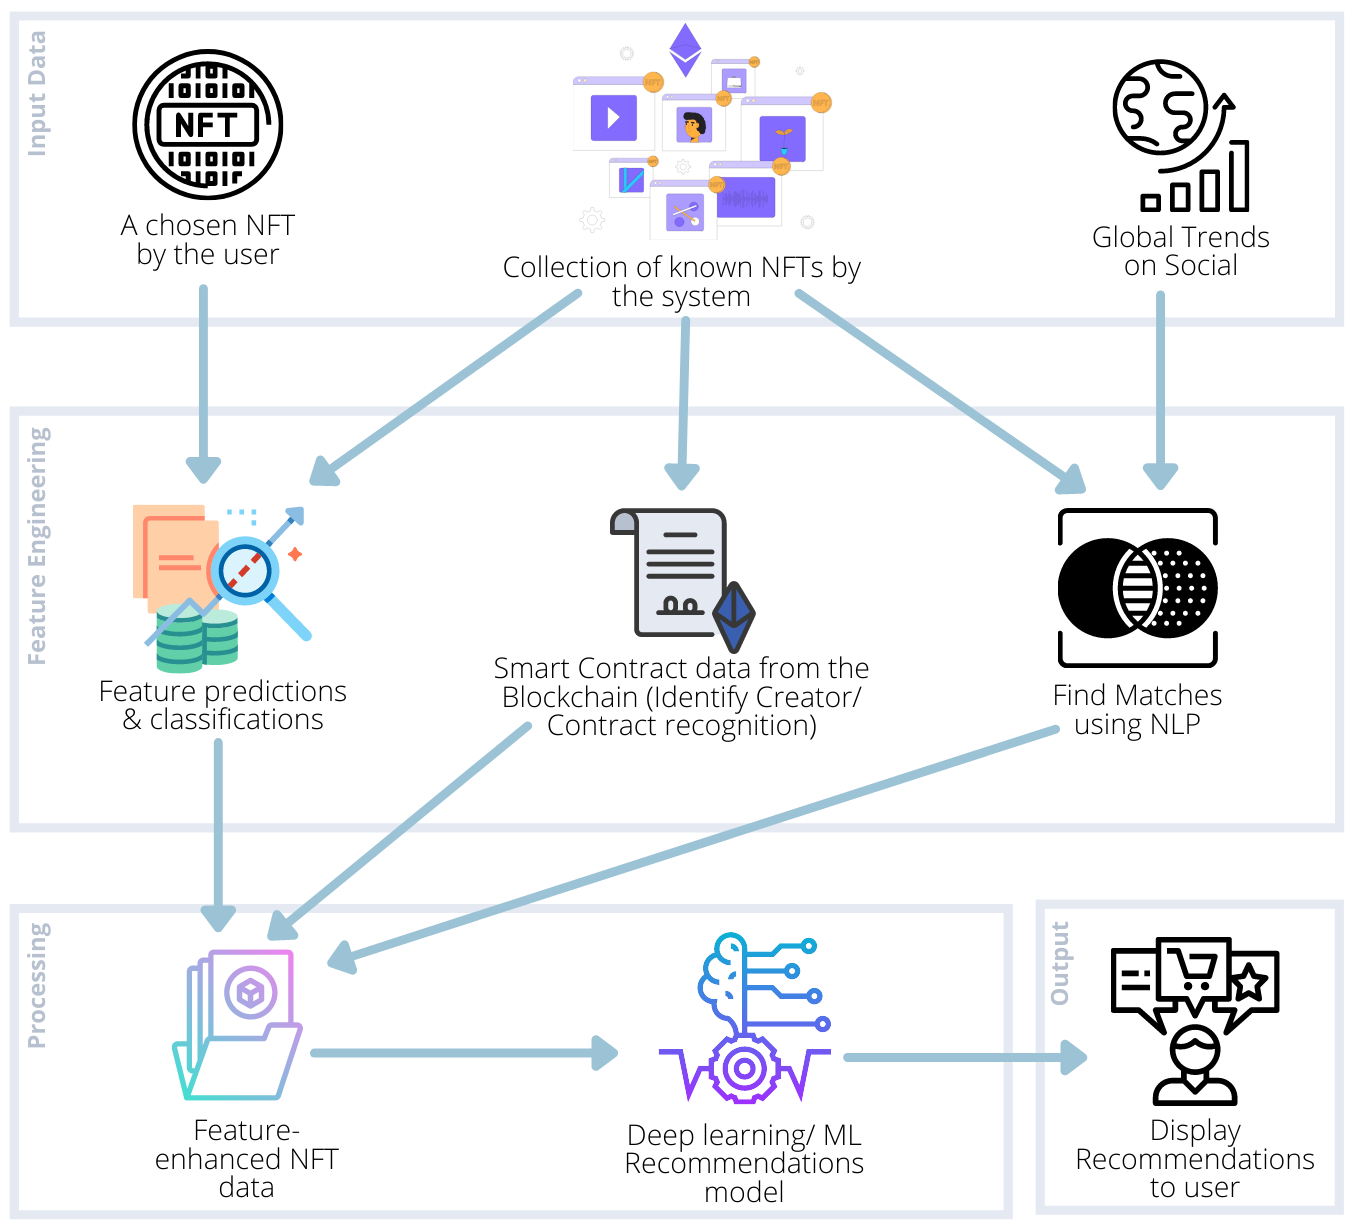
\includegraphics[height=0.5\textheight]{images/prototype-feature-diagram.png}
% \vspace{-7mm}       % remove spacing
\caption{Prototype Feature Diagram \textit{(self-composed)}}
\end{figure}

\vspace{-4mm}
\section{Chapter Summary}
This chapter presented the problem with necessary proofs and domain description, the research gap, the research challenge, and the research strategy that is expected to be addressed by the author in the research project presented by this document. The research objectives were mapped to the learning outcomes of the project module in the BSc(Hons) Computer Science undergraduate program of the University of Westminster.